% xelatex
% vim:set et sw=4 ts=4 tw=80:
% \documentclass[12pt]{apa7}
\documentclass[12pt]{report}

\usepackage{pdfpages}
\usepackage{setspace}
\usepackage{fontspec}
\usepackage[a4paper, margin=1in]{geometry}
\usepackage{blindtext}
\usepackage{indentfirst}
\usepackage[
    backend=biber,
    style=apa,
    defernumbers=true,
]{biblatex}
\addbibresource{report.bib}
\usepackage{hyperref}
\usepackage{kantlipsum}
\usepackage{lipsum}
\usepackage{graphicx}
% \usepackage{hologo}
\usepackage{pgfplots}
\usepackage{tikz,tikz-3dplot}
\usepackage{float}
\usepackage{multicol}
\usepackage{enumitem}
\usepackage{amsmath}
% \usepackage{datatool}
% \DTLloaddb{data}{data/data-nums.csv}
\usepackage{pgf-pie}  

\pgfplotsset{compat=newest}
% \usepgfplotslibrary{external}
% \tikzexternalize


\setstretch{1.15}
\setmainfont{Times New Roman}
\pagenumbering{roman}
\title{Comparing the Qualitative Effects Between Procrastination and Family
Pressure on Exam Anxiety}
\author{
    Marawan MogebElrahman Foud AbdElbaset \\
    \texttt{\href{mailto:marawan.1519030@stemluxor.moe.edu.eg}{marawan.1519030@stemluxor.moe.edu.eg}} \\
    SalahDin Ahmed Salh Rezk \\
    \texttt{\href{mailto:salahdin.1519013@stemluxor.moe.edu.eg}{salahdin.1519013@stemluxor.moe.edu.eg}} \\
    Younis Tarek Hanafi Metwaly \\
    \texttt{\href{mailto:younis.1519035@stemluxor.moe.edu.eg}{younis.1519035@stemluxor.moe.edu.eg}} \\
    \\\\
    Luxor STEM School
    \includegraphics[height=.85em]{images/luxor.jpg}
    and
    Qena STEM School
    \includegraphics[height=.85em]{images/qena.png}
    \\
    under the Egyptian Ministry of Education
    \includegraphics[height=.85em]{images/ministry.png}
    \\\\
    English Class Grade 12
    \\\\
    Mr. Khalil
    % \href{mailto:khalil@stemqena.moe.edu.eg}{{\fontspec{Symbola}\char"1F4E7}}
}
\date{\today}

\renewcommand{\abstractname}{Executive Summary}
\tikzset{
    legend to the south/.code={
        \coordinate[
        xshift=-1.5cm,
        yshift=0
        ] (legendpos) at
    (current bounding box.south);},
}

\begin{document}
\maketitle
\tableofcontents
\listoffigures
% \listoftables

\begin{abstract}
    
    Exam anxiety is a huge factor in the daily life of students. It may affect
    their possible performance in exams resulting in an undesirable future. The
    most common causes of exam anxiety are the lack of preparation and family
    pressure. This report presents the qualitative effects of two in order to
    form more sophisticated plans for dealing with the educational issues they
    arises. The method by which these factors are compared is based on a
    3-dimensional 10-point scale which input is an 8-question survey. The test
    was done on a sample of 44 Egyptian students ranging from 15 to 22 years
    old. The model concluded that family pressure has more effect than
    procrastination on exam anxiety by 40\%. Additionally, it was possible to
    deduce that a problem-specific—based strategy is the most suitable to deal
    with exam anxiety. However, the results are not conclusive since the study
    did not take into account external factors that might affect the system.
    
    \addcontentsline{toc}{chapter}{Executive Summary}
    \thispagestyle{plain}
    \pagenumbering{arabic}
\end{abstract}

\chapter{Introduction}
\setcounter{page}{2}
\begin{multicols}{2}
\section{Problem}

It is a notable phenomenon that individuals do experience some kind of anxiety
throughout their life — especially their academic one — increasing the
probability of mistakes during most critical tasks. It is usually the case that
such seemingly useless traits affecting people's day-to-day life has some kind
of an advantage to humans' ancestors \parencite{Price2003-bl}. 

Anxiety can be described as the tense, unsettling anticipation of a threatening
but vague event \parencite{Rachman2019-cn}. There are two distinct types of
anxiety: objective and neurotic. Fear is usually considered as a type of
objective anxiety, while neurotic anxiety is a product of internal perceptions
and emotions \parencite{Spielberger1966-dk}. 

According to \cite{mowrer1939stimulus}, neurotic anxiety is defined as a result
of the act which an individual commits to but wishes they had not. This
definition does explain the frequency of such a feeling; this can be noticed
through most modern subcategories of anxiety (e.g. exam anxiety, marriage
anxiety, etc).

Attention should be directed towards the field of education due to its flexible
nature compared to other professional fields, also it is the foundation for
every single considerable profession. The main type of anxiety concerning this
field is exam anxiety \parencite{academic-anxiety}, ergo the focus of this study.

\cite{rana_2010_the} describes the effect of cognitive factors (i.e worry) on
academic performance of the students. The impact of anxiety was indisputable;
the worry scale had the greatest correlation with the students' performance
compared to all other measured scales. In addition, \cite{trifoni2011does} works
on different scales relating to anxiety, one illustrates the students'
opinions on the topic: students who were more anxious had more radical opinions
concerning the subject compared to their less anxious peers.

\section{Hypothesis}

The main focus of the study is the effects of procrastination and family
pressure on exam anxiety. Accordingly, the proposed hypothesis is that
procrastination does have a higher effect than that of family pressure. The
importance of such a hypothesis may not seem clear at first; however, the result
will determine which should be the concern of a family dealing with their
children. \textit{``Should I change the way I am supporting my kid or force him
to study more and avoid procrastination?"} is the kind of questions that this
research try to answer effectively.

\end{multicols}

\chapter{Body}
\begin{multicols}{2}
    
\section{Methodology}

\subsection{Sample}

The sample mainly consisted of randomized students ranging from high school to
university. The students were from different geographic areas, different
schools, and different systems of education. The sample was taken from the
Egyptian internet population, so the results will be limited to the Egyptian
population at best. The age of the students ranged from 15 to 22; although there
were some outliers ranging from 30 to 49. The gender was not collected due to
its overall insignificant effect on the results \parencite{hashmat2008factors}.

\subsection{Questions}

\begin{enumerate}[wide, labelwidth=!, labelindent=0pt]

    \item \textit{How much did procrastination affect your academic performance?}
\textbf{(10-point scale)}

This question measures the effect of procrastination on performance from the
student's perspective, essentially measuring the amount of procrastination while
avoiding the feeling of guilt this question usually results in.

\item \textit{How harsh did your family go on you to study last year?}
\textbf{(10-point scale)}

This question measures the amount of family pressure a student has endured
without implicitly mentioning family pressure to avoid bias caused by family
relations by mentioning it more as a beneficial parental act.

\item \textit{How satisfied were you with your last year's academic
performance?}
\textbf{(10-point scale)}

This question measures the student's satisfaction with their academic
performance in order to correlate it with procrastination and family pressure.

\item \textit{How stressful did you feel about last year's exams?}
\textbf{(10-point scale)}

This question measures the student's stress factor, which affects exam anxiety
the most, in order to correlate it with procrastination and family pressure.

\item \textit{How hard it takes you to recover after bad grades?}
\textbf{(open-ended)}

This question tries to find the relation between the amount of exam anxiety
and the recovering factor.

\item \textit{What are the factors that lead to exam anxiety from your
perspective?}
\textbf{(open-ended)}

This questions collects other factors that may affect or be affected by family
pressure, procrastination, or both. This may even help in drawing conclusions
beyond the scope of this study.

\item \textit{How do you get ready mentally for your exams?}
\textbf{(open-ended)}

This question tries to find solutions provided by students and correlate them
with the amount of exam anxiety in order to measure their effectiveness.

\item \textit{Which affected your performance the most?}
\textbf{(multiple choices)}

This question tests a student's perspective of their situation to enable comparing
what students think with the calculated results of other questions.

\end{enumerate}

\section{Findings}

There is a notable correlation between both family pressure and procrastination
seen in Figure~\ref{fig:procrastination-stress} and
Figure~\ref{fig:family-stress}. Despite that, there is a weak correlation in
Figure~\ref{fig:procrastination-family} that may hint to problems within this
model. Thus, a more sophisticated tool should be formulated; accordingly, the
exam anxiety factor ($EA$) is defined in Equation~\ref{eq:exam-anxiety}.

A 3-dimensional plot of the exam anxiety could be helpful in demonstrating
the relation between procrastination and family pressure. Figure~\ref{fig:3d}
shows a greater correlation between the two factors and exam anxiety, but family
pressure is clearly more dominant. The increase of both factors results in a
noticeable increase in exam anxiety.

The best fit curve for family pressure ($F$) and procrastination ($P$) are
Equation~\ref{eq:eaf-f} and Equation~\ref{eq:eaf-p} respectively with
determination coefficients of $R^2 = 0.04$ and $R^2 = 0.06$.

\begin{equation}
    EAF = \textnormal{stress} -
    \frac{\textnormal{satisfaction}}{\textnormal{recovery}}
    \label{eq:exam-anxiety}
\end{equation}

\begin{figure}[H]
    \begin{tikzpicture}
        \begin{axis}[
            width = \linewidth,
            only marks,
            mark size=3pt,
            scatter,
            xlabel = procrastination,
            ylabel = stress,
            legend style={
                at={(0.44,-0.2)},
                anchor=north,legend columns=-1
            },
            grid style=dashed,
            ymajorgrids=true,
            xmajorgrids=true,
            ]
            \addplot[] table [
                x=procrastination,
                y=stress,
                col sep=comma
                ]{data/data-nums.csv};
        \end{axis}
    \end{tikzpicture}
    \caption{Procrastination versus stress plot}
    \label{fig:procrastination-stress}
\end{figure}

\begin{figure}[H]
    \begin{tikzpicture}
        \begin{axis}[
            width = \linewidth,
            only marks,
            mark size=3pt,
            scatter,
            xlabel = family pressure,
            ylabel = stress,
            legend style={
                at={(0.44,-0.2)},
                anchor=north,legend columns=-1
            },
            grid style=dashed,
            ymajorgrids=true,
            xmajorgrids=true,
            ]
            \addplot[] table [
                x=family,
                y=stress,
                col sep=comma
                ]{data/data-nums.csv};
        \end{axis}
    \end{tikzpicture}
    \caption{Family pressure versus stress plot}
    \label{fig:family-stress}
\end{figure}

\begin{figure}[H]
    \begin{tikzpicture}
        \begin{axis}[
            width = \linewidth,
            only marks,
            mark size=3pt,
            scatter,
            xlabel = procrastination,
            ylabel = family pressure,
            legend style={
                at={(0.44,-0.2)},
                anchor=north,legend columns=-1
            },
            grid style=dashed,
            ymajorgrids=true,
            xmajorgrids=true,
            ]
            \addplot[] table [
                x=procrastination,
                y=family,
                col sep=comma
                ]{data/data-nums.csv};
        \end{axis}
    \end{tikzpicture}
    \caption{Procrastination versus family pressure plot}
    \label{fig:procrastination-family}
\end{figure}

\begin{align}
    \label{eq:eaf-f}
    EA &= 0.027 F^3 - 0.4 F^2 + 1.6 F + 3\\
       \label{eq:eaf-p}
       &= -0.20 P^2 + 2.7 P - 2.7\\
       \label{eq:eaf-fp}
       &= 0.18 F - 0.20 P + 5.6
\end{align}

Despite that, the unmatching Equation~\ref{eq:eaf-fp} has a determination
coefficient $R^2 = 0.024$, which may indicate that the two factors have a strong
mutual impact on exam anxiety. Additionally, these equations indicate that,
while procrastination has a larger effect, it does not stay as long as family
pressure, and after a specific critical point ($P=7$) its effect starts
declining.

On the other hand, Figure~\ref{fig:bar} shows the total of exam anxiety across
age groups. The bar chart shows a clear increase around the age of 17, which is
the average age for high school seniors. This reflects the large importance that
the Egyptian society puts on this year resulting in an increase in exam anxiety.
At the age of 20 students tend to be more anxious than at the age of 15,
although there is less pressure on their academic life as they are in college.
This may indicate that other factors take effect on exam anxiety later on in
life.

Following students' awareness of the problem, the pie chart in
Figure~\ref{fig:pie} shows the percentage of students' ideas of the most
problematic aspect of their life. This shows a clear bias towards
procrastination. It is possible that the cause of such bias is the constructs of
modern society. 

Finally, the factors of exam anxiety and the methods to avoid it were closely
related to each other. Students who tend to be lazier had better techniques for dealing with procrastination while students who tend to be more pressured had better techniques for dealing with external factors.

\begin{figure}[H]
    \begin{center}
        \begin{tikzpicture}[scale=0.9, transform shape]
            \begin{axis}[
                width = \linewidth,
                mark size=2.7pt,
                zlabel = exam anxiety,
                grid style=dashed,
                ymajorgrids=true,
                xmajorgrids=true,
                zmajorgrids=true,
                zlabel style={sloped},
                clip=false,
                ]
                \addplot3[
                    scatter,
                    only marks,
                    ] table [
                    x=procrastination,
                    y=family,
                    z=EAF,
                    col sep=comma,
                    ]{data/data-nums.csv};
                \node at (rel axis cs:0,0.4,1.1) [above,sloped like y axis] {family
                    pressure};
                \node at (rel axis cs:1,0,1.7) [above,sloped like x axis]
                    {procrastination};

            \end{axis}
        \end{tikzpicture}
    \end{center}
    \vspace*{-5mm}
    \caption{Exam anxiety plot}
    \label{fig:3d}
\end{figure}

\begin{figure}[H]
    \center
        \begin{tikzpicture}[scale=0.9, transform shape]
            \begin{axis}[
                ybar stacked,
                xlabel=age,
                ylabel=total exam anxiety,
                ]
                \addplot+[
                    ybar,
                    ] table[
                    x=age,
                    y=sum EAF,
                    col sep=comma,
                    ] {data/bar.csv};
            \end{axis}
        \end{tikzpicture}
    \caption{Bar chart of exam anxiety by age}
    \label{fig:bar}
\end{figure}

\begin{figure}[H]
    \center
    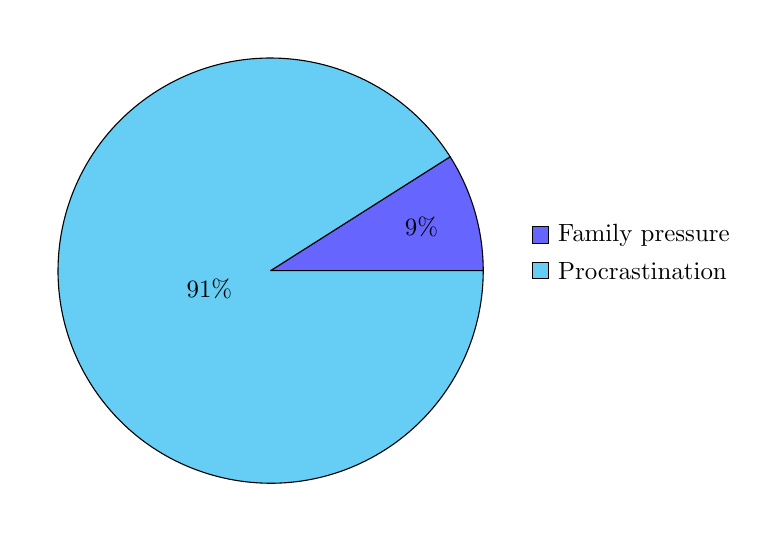
\begin{tikzpicture}[scale=0.9, transform shape]
        \pie[
        text=legend,
        style={legend to the south},
        ]{
            9/Family pressure,
            91/Procrastination
        }
    \end{tikzpicture}
    \vspace*{-1mm}
    \caption{Pie chart of students' perspective}
    \label{fig:pie}
\end{figure}

\end{multicols}

\chapter{Conclusion}
\begin{multicols}{2}

\section{Summary of Findings}

The previous analysis showed that the factors of exam anxiety (i.e.
procrastination and family pressure) are related to each other in such a way
that the two affect both each other and the exam anxiety; no one factor can be
analyzed independently, which raises the possibility of other relating factors.
The most prominent factor is the family pressure, which rejects the proposed
hypothesis of procrastination being of a greater effect. In fact, it had an
effect of 39.53\% greater than procrastination.

The result is unexpected due to the clear problem that procrastination creates
and the fact that the family implies that students get stressed more by
expectations from those around them than the catastrophic failures they may be
the cause of. Moreover, procrastination had a peak value for affecting exam
anxiety while family pressure had not.

On the other hand, there is an expected variation in exam anxiety among
different age groups of students. Students who are around their senior high
school year tend to be more anxious due to the increase in family pressure.
Furthermore, students at the age of 17 are, on average, twice as anxious as
their peers. 

While it is indubitable, by this point, that family pressure is the player
factor in this game. Students tend to underestimates its effect on exam anxiety.
91\% of the students reported that the majority of their pressure was caused by
procrastination, although it was concluded to be only 40\% of the total.

\section{Recommendations}

The problem at hand is hard to solve. However, it is possible to reach
reasonable conclusions from the data and answers. The most notable pattern in
less anxious students is their awareness of the most prominent factor affecting
them. They know what the problem is and then solve it. Each aware student had
their own technique for dealing with their anxiety. The techniques are not the
same yet they fall in similar categories.

The main category that helped with family pressure was health care (e.g.
hydration, exercise, etc) while the main one that helped with procrastination
was self-control (e.g. scheduling, prioritizing, etc). Students who tried to
deal with procrastination with a strategy of family pressure or vice versa had
higher anxiety.

The solution proposed based on the data is a multi-step process that is most
concerned with the identification of the anxiety type, then applying a number
of actions proved to be effective with this type.

\end{multicols}

\printbibliography[heading=bibintoc, title={References}]

\appendix
\chapter{Questionnaire}
% \includepdf{questionnaire}

\begin{center}
    % \makebox[\textwidth][c]{\includegraphics[width=1.05\textwidth] {questionnaire.pdf}}
    \includegraphics[width=1\linewidth]{questionnaire.pdf}
\end{center}

% \chapter{Technical Notes}
% This document was completely made within {\LaTeX} markup language for
% typesetting with \hologo{BibTeX} for bibliography using an external text editor
% i.e. NeoVIM while managing version revisions and teamwork with Git.

\end{document}
